\documentclass[11pt]{article}

\usepackage[margin=0.78in]{geometry}
\usepackage{amsmath,amssymb}
\usepackage{booktabs,array,tabularx,textcomp}
\usepackage{graphicx}
\usepackage{microtype}
\usepackage{xcolor}
\usepackage{hyperref}
\usepackage{caption}
\usepackage{float}
\usepackage{enumitem}

\definecolor{accent}{HTML}{245A7A}
\hypersetup{
  colorlinks=true,
  linkcolor=accent,
  urlcolor=accent,
  citecolor=accent
}
\captionsetup{font=small,labelfont=bf}
\setlist{nosep,leftmargin=*}
\setlength{\parindent}{0pt}
\setlength{\parskip}{0.45em}

\newcommand{\studentname}{Don van Beusichem}
\newcommand{\notebookurl}{https://colab.research.google.com/drive/1IhZVrHby1eqb0qL0XkNx7c4TMkqqj1jG}

\title{\vspace{-1.6em}\textbf{PHYS 2550 Homework 2}}
\author{\studentname}
\date{October 15, 2026}

\setlength{\emergencystretch}{2em}
\begin{document}
\maketitle
\vspace{-1.7em}
\begin{center}
\href{\notebookurl}{\texttt{Colab notebook}}
\end{center}
\section{Theory}

\subsubsection*{T1. Counting parameters.}

For a dense layer with $n$ inputs and $m$ outputs, I count $(n+1)m$ parameters. For a convolution, the count is $(k^2C_{\mathrm{in}}+1)C_{\mathrm{out}}$. The extra term is the bias, counted once per output. ReLU, pooling, flattening and dropout do not add trainable parameters.


\begin{table}[H]\centering
\caption{Parameter counts for the three reference architectures.}
\small
\begin{tabular}{@{}>{\raggedright\arraybackslash}p{\dimexpr 0.335308\linewidth-8.047pt\relax}>{\raggedright\arraybackslash}p{\dimexpr 0.483227\linewidth-11.597pt\relax}>{\raggedright\arraybackslash}p{\dimexpr 0.181465\linewidth-4.355pt\relax}@{}}
\toprule
Model / layer & Calculation & Parameters \\
\midrule
CNN: convolution 1 & (3 \ensuremath{\times} 3 \ensuremath{\times} 3 + 1) \ensuremath{\times} 16 & 448 \\
CNN: convolution 2 & (3 \ensuremath{\times} 3 \ensuremath{\times} 16 + 1) \ensuremath{\times} 32 & 4,640 \\
CNN: convolution 3 & (3 \ensuremath{\times} 3 \ensuremath{\times} 32 + 1) \ensuremath{\times} 64 & 18,496 \\
CNN: dense 64 & (6 \ensuremath{\times} 6 \ensuremath{\times} 64 + 1) \ensuremath{\times} 64 & 147,520 \\
CNN: output & (64 + 1) \ensuremath{\times} 10 & 650 \\
\textbf{CNN total} &  & \textbf{171,754} \\
FCNN-matched: dense 24 & (6,912 + 1) \ensuremath{\times} 24 & 165,912 \\
FCNN-matched: dense 64 & (24 + 1) \ensuremath{\times} 64 & 1,600 \\
FCNN-matched: output & (64 + 1) \ensuremath{\times} 10 & 650 \\
\textbf{FCNN-matched total} &  & \textbf{168,162} \\
FCNN-large: dense 256 & (6,912 + 1) \ensuremath{\times} 256 & 1,769,728 \\
FCNN-large: dense 128 & (256 + 1) \ensuremath{\times} 128 & 32,896 \\
FCNN-large: output & (128 + 1) \ensuremath{\times} 10 & 1,290 \\
\textbf{FCNN-large total} &  & \textbf{1,803,914} \\
\bottomrule
\end{tabular}
\end{table}

Most of the CNN's parameters are actually in its first dense layer: $147{,}520/171{,}754 \approx 85.9\%$. In the FCNN, each first-layer node connects to all 6,912 input values and needs 6,913 parameters including its bias. Just 24 nodes therefore use 165,912 parameters. This leaves the matched FCNN only about 2.1\% smaller than the CNN; a wider first layer would quickly exceed that budget.

\subsubsection*{T2. Convolution and pooling by hand.}

\textbf{(a)} For the upper-left entry, I get $5(3)-2-0-1-1=11$. Repeating this across the input gives a $3\times3$ map:
\begin{equation}
I\star K=\begin{bmatrix}11&-4&6\\-4&15&-4\\-5&2&9\end{bmatrix}.
\end{equation}

\textbf{(b)} For dilation 1, I use
\begin{equation}
N_{\mathrm{out}}=\left\lfloor\frac{N+2p-k}{s}\right\rfloor+1.
\end{equation}
Padding 1 therefore gives $5\times5$, while stride 2 without padding gives $2\times2$.

\textbf{(c)} Applying $2\times2$ pooling with stride 1, I get
\begin{equation}
M=\begin{bmatrix}15&15\\15&15\end{bmatrix},\qquad
A=\begin{bmatrix}4.50&3.25\\2.00&5.50\end{bmatrix}.
\end{equation}
For example, the upper-left average is $(11-4-4+15)/4=4.5$.

If I move the bright central pixel, its sharpened response and the responses around it change. Max pooling can keep the same peak while it stays inside a window. Once it crosses a window boundary, that need not hold. Average pooling spreads the change across overlapping windows, so neither map is exactly invariant to the movement.

\textbf{(d)} The kernel entries sum to one, so a constant intensity $c$ stays unchanged away from the boundaries. For independent noise, I get
\begin{equation}
\mathrm{Var}(I\star K)=\sigma^2\sum K^2=29\sigma^2.
\end{equation}
The noise standard deviation therefore increases by $\sqrt{29}\approx5.39$. Sharpening may make an edge clearer, but it also greatly amplifies the sky noise. I would be careful about using it on faint galaxies.

\textbf{(e)} This kernel is unchanged by a 180\textdegree{} flip, so convolution and cross-correlation give the same result. For a learned kernel, flipping simply relabels the trainable coefficients: either convention represents the same family of functions. The numerical arrays of learned weights need not be identical.

\subsubsection*{T3. Shapes and receptive field.}

\textbf{(a)} Following the input through the CNN gives the shapes below.


\begin{table}[H]\centering
\caption{Layer shapes and receptive fields.}
\small
\begin{tabular}{@{}>{\raggedright\arraybackslash}p{\dimexpr 0.335308\linewidth-8.047pt\relax}>{\raggedright\arraybackslash}p{\dimexpr 0.355032\linewidth-8.521pt\relax}>{\raggedright\arraybackslash}p{\dimexpr 0.309660\linewidth-7.432pt\relax}@{}}
\toprule
Layer & Output shape H \ensuremath{\times} W \ensuremath{\times} C & Receptive field / jump \\
\midrule
Input & 48 \ensuremath{\times} 48 \ensuremath{\times} 3 & 1 / 1 \\
Conv 1; ReLU & 48 \ensuremath{\times} 48 \ensuremath{\times} 16 (each) & 3 / 1 \\
Pool 1 & 24 \ensuremath{\times} 24 \ensuremath{\times} 16 & 4 / 2 \\
Conv 2; ReLU & 24 \ensuremath{\times} 24 \ensuremath{\times} 32 (each) & 8 / 2 \\
Pool 2 & 12 \ensuremath{\times} 12 \ensuremath{\times} 32 & 10 / 4 \\
Conv 3; ReLU & 12 \ensuremath{\times} 12 \ensuremath{\times} 64 (each) & 18 / 4 \\
Pool 3 & 6 \ensuremath{\times} 6 \ensuremath{\times} 64 & 22 / 8 \\
Flatten & 2,304 values & All locations retained \\
Dense 64; ReLU; dropout & 64 values (each) & Global combination \\
Dense output & 10 logits & Global combination \\
\bottomrule
\end{tabular}
\end{table}

\textbf{(b)} For kernel size $k$ and stride $s$, the receptive field $r$ and spacing $j$ follow
\begin{equation}
r'=r+(k-1)j,\qquad j'=sj.
\end{equation}
A unit after the third convolution sees $18\times18$ input pixels, smaller than a typical 20--40 pixel galaxy. The final pooling layer reaches $22\times22$, which can cover a small, suitably aligned galaxy but not a 40-pixel one. The dense head combines features across the whole crop.

\textbf{(c)} A first convolution with stride 2 and no padding would produce $23\times23\times16$.

\subsubsection*{T4. Equivariance and invariance.}

\textbf{(a)} Translation equivariance means that shifting the input shifts the output in the same way, $f(T_\delta x)=T_\delta f(x)$. Invariance means that the output stays unchanged, $f(T_\delta x)=f(x)$. Ignoring boundaries,
\begin{equation}
[K\star T_\delta x](u)=\sum_v K(v)x(u+v-\delta)
=[T_\delta(K\star x)](u).
\end{equation}
Shared convolutional weights therefore give translation equivariance, and pointwise ReLU preserves it.

\textbf{(b)} Pooling reduces sensitivity to small local shifts. However, its stride and window boundaries, image padding, and the position-dependent dense head prevent exact invariance. Dropout does not itself enforce translation invariance.

\textbf{(c)} An unconstrained FCNN has separate weights for each input position, so neither property is built in. I expect both models to lose accuracy when I shift the crops, but I expect the CNN's drop to be smaller.

\subsubsection*{T5. Scrambled pixels.}

A fixed permutation preserves every pixel value but changes its neighbours. An FCNN can absorb this reordering into the columns of its first weight matrix, so its representational capacity is unchanged. After retraining, I expect similar performance within optimisation and seed variation. A CNN's small kernels instead act on pixels that are no longer spatial neighbours. I expect its advantage to shrink. Scrambling tests the usefulness of locality, rather than simply removing information from the input.

\subsubsection*{T6. Parameters are not compute.}

\textbf{(a)} I counted one MAC per input--weight pair in each output. The totals are:


\begin{table}[H]\centering
\caption{Forward multiply--accumulate counts.}
\small
\begin{tabular}{@{}>{\raggedright\arraybackslash}p{\dimexpr 0.414204\linewidth-9.941pt\relax}>{\raggedright\arraybackslash}p{\dimexpr 0.309660\linewidth-7.432pt\relax}>{\raggedright\arraybackslash}p{\dimexpr 0.276136\linewidth-6.627pt\relax}@{}}
\toprule
Forward operation & CNN MACs & FCNN-matched MACs \\
\midrule
First layer & 48\textsuperscript{2} \ensuremath{\times} 16 \ensuremath{\times} 27 = 995,328 & 6,912 \ensuremath{\times} 24 = 165,888 \\
Second layer & 24\textsuperscript{2} \ensuremath{\times} 32 \ensuremath{\times} 144 = 2,654,208 & 24 \ensuremath{\times} 64 = 1,536 \\
Third convolution & 12\textsuperscript{2} \ensuremath{\times} 64 \ensuremath{\times} 288 = 2,654,208 & --- \\
Dense head & 2,304 \ensuremath{\times} 64 + 64 \ensuremath{\times} 10 = 148,096 & 64 \ensuremath{\times} 10 = 640 \\
\textbf{Total} & \textbf{6,451,840} & \textbf{168,064} \\
\bottomrule
\end{tabular}
\end{table}

\textbf{(b)} I get about 38.4 times as many forward MACs for the CNN as for FCNN-matched. It reuses each convolutional weight at many positions, saving parameters without eliminating the corresponding multiplications. Training also requires backward operations and parameter updates, so 38.4 is an arithmetic estimate, not an exact wall-clock ratio. Hardware, batching and memory access affect the measured ratio. FCNN-large requires 1,803,520 forward MACs.

\textbf{(c)} A CNN could still reach a given validation accuracy in fewer epochs. Whether that also means less time depends on how expensive each epoch is. I therefore compare seconds per epoch, epochs to the same target, and total seconds to that target, including how many runs never reach it.

\subsubsection*{T7. Pooling and noise.}

\textbf{(a)} Averaging four independent sky pixels gives mean $\mu$ and variance $4\sigma^2/16=\sigma^2/4$. The output standard deviation is therefore $\sigma/2$.

\textbf{(b)} Max pooling is biased upward. For Gaussian noise, its expected output is approximately $\mu+1.03\sigma$, so it can select a positive fluctuation even when there is no source.

\textbf{(c)} For a dark object on a light background, min pooling would preserve the dark response more naturally than max pooling. For a faint, extended galaxy on noisy sky, I would consider average pooling in the first layer because it reduces independent noise while preserving a local mean signal. It can also dilute small bright features. The prescribed comparison retains max pooling in all three blocks; changing it would change the reference architecture. Moreover, a learned feature map is not raw sky, and the independent-noise calculation is only an approximation there.

\subsubsection*{T8. Reading training curves.}

\textbf{(a)} In the supplied curves, I can see that FCNN-large is overfitting: training loss keeps falling while validation loss reaches a minimum near epoch 8 and then rises. I would select that minimum with early stopping. The CNN has a much smaller gap and both curves flatten together, with no clear severe overfitting. That does not tell me its remaining error is unavoidable.

\textbf{(b)} Weight decay discourages large weights and reduces model flexibility. Increasing dropout makes the network less dependent on particular hidden units. Both can reduce the FCNN's gap, but excessive regularisation can cause underfitting. 

\textbf{(c)} The CNN's local connections and shared weights constrain the functions it can learn in a way suited to images. That helps explain a smaller gap; seeing the same training images does not give two architectures the same generalisation behaviour.


\section{Data and preprocessing}

\subsection{First look}

The file contains 21,785 images of shape 69 \ensuremath{\times} 69 \ensuremath{\times} 3, stored as uint8, with pixel values from 0 to 255. The label array has one integer per image. I used Galaxy10 SDSS, whose labels are derived from Galaxy Zoo votes \cite{ref1}. A fixed seed of 2550 gives 15,249 training, 3,268 validation and 3,268 test images, using a stratified 70/15/15 split.


\begin{table}[H]\centering
\caption{Class counts and the stratified data split.}
\footnotesize
\begin{tabular}{@{}>{\raggedright\arraybackslash}p{\dimexpr 0.069034\linewidth-4.142pt\relax}>{\raggedright\arraybackslash}p{\dimexpr 0.477310\linewidth-28.639pt\relax}>{\raggedright\arraybackslash}p{\dimexpr 0.118345\linewidth-7.101pt\relax}>{\raggedright\arraybackslash}p{\dimexpr 0.118345\linewidth-7.101pt\relax}>{\raggedright\arraybackslash}p{\dimexpr 0.108483\linewidth-6.509pt\relax}>{\raggedright\arraybackslash}p{\dimexpr 0.108483\linewidth-6.509pt\relax}@{}}
\toprule
Class & Morphology & All & Train & Val. & Test \\
\midrule
0 & Face-on, no spiral & 3461 & 2423 & 519 & 519 \\
1 & Smooth, round & 6997 & 4898 & 1049 & 1050 \\
2 & Smooth, intermediate & 6292 & 4404 & 944 & 944 \\
3 & Smooth, cigar & 349 & 244 & 52 & 53 \\
4 & Edge-on, rounded bulge & 1534 & 1074 & 230 & 230 \\
5 & Edge-on, boxy bulge & 17 & 12 & 3 & 2 \\
6 & Edge-on, no bulge & 589 & 412 & 89 & 88 \\
7 & Tight spiral & 1121 & 785 & 168 & 168 \\
8 & Medium spiral & 906 & 634 & 136 & 136 \\
9 & Loose spiral & 519 & 363 & 78 & 78 \\
\bottomrule
\end{tabular}
\end{table}

I kept all ten classes to preserve the supplied reference models. Class 5 has only 17 examples, so its measured recall is highly uncertain; classes 3, 6 and 9 are also relatively uncommon. The verified file has 349 class-3 images, rather than the 394 listed in the documentation. I use the measured count. I report balanced accuracy, the mean of ten class recalls, alongside accuracy; it exposes minority-class failures but also gives the tiny class considerable influence.


\begin{figure}[H]
\centering
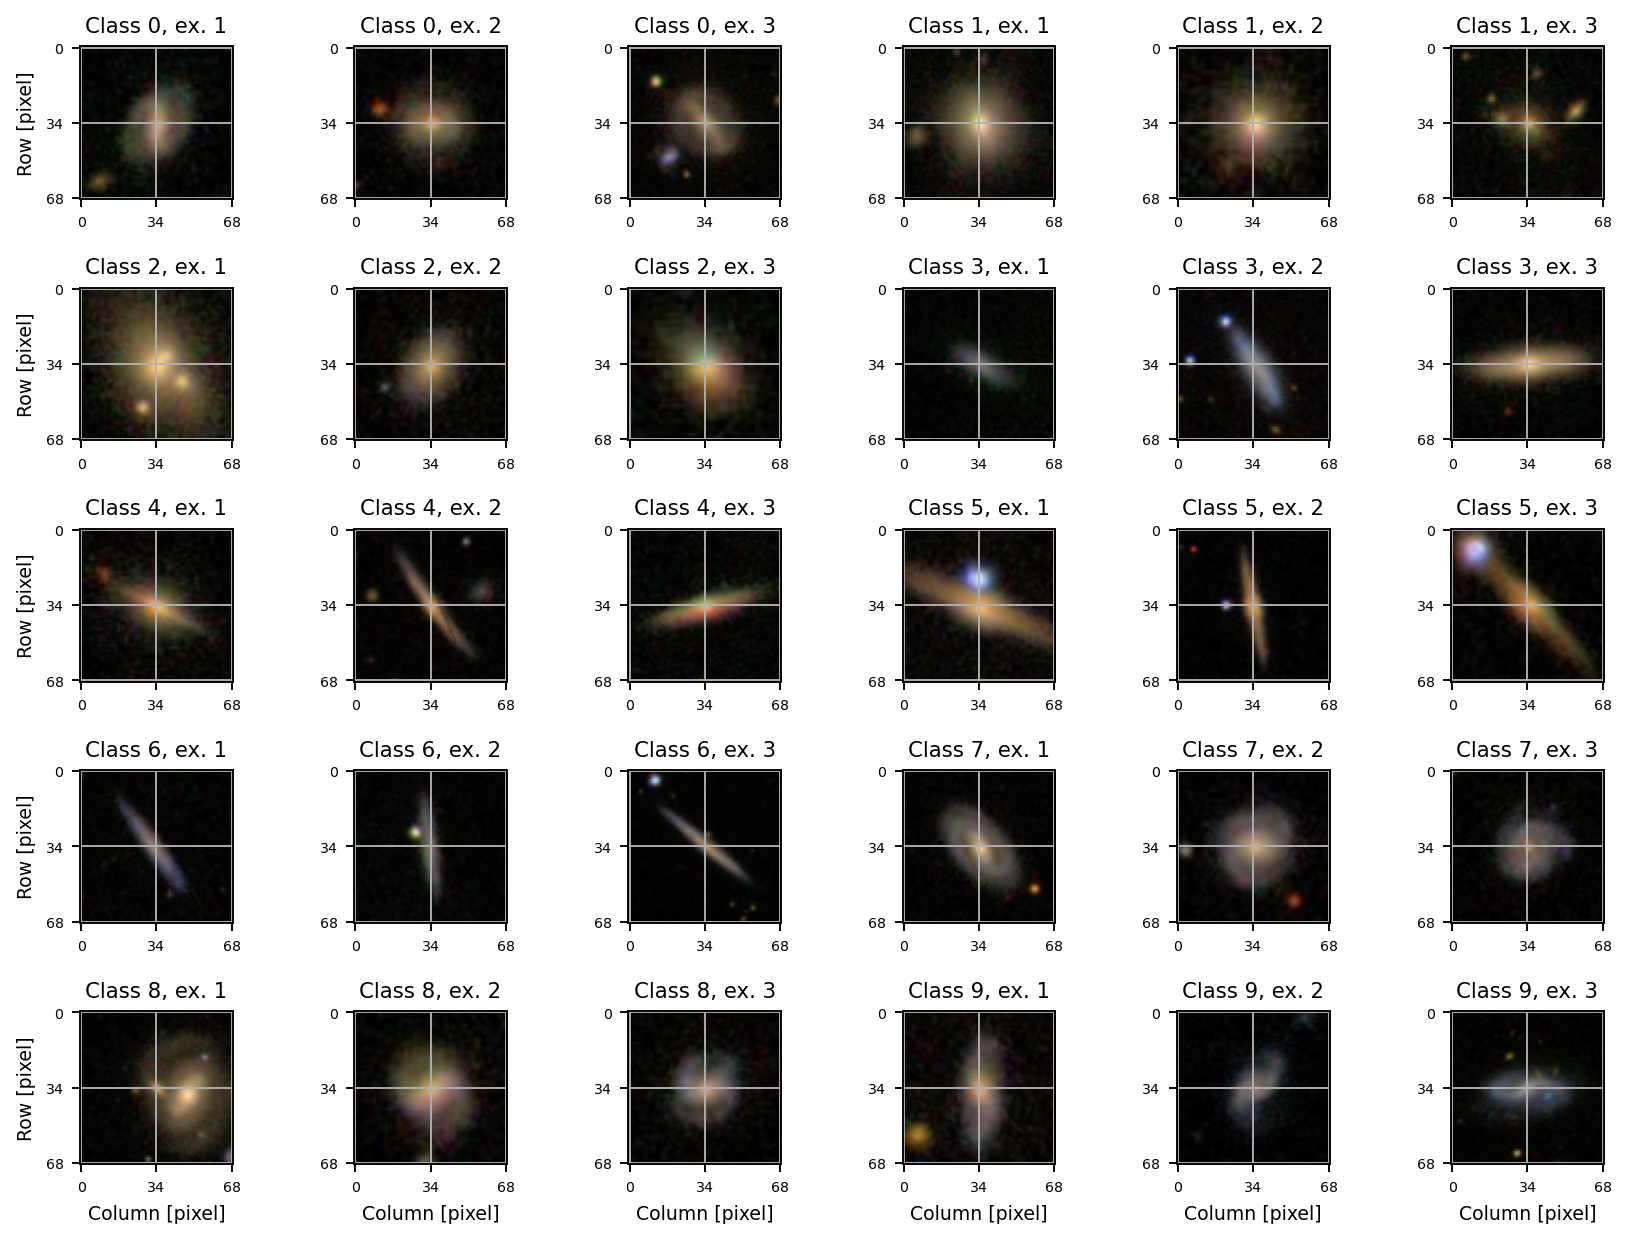
\includegraphics[width=0.94\linewidth,height=335pt,keepaspectratio]{figures/class_examples.png}
\caption{Three training examples per class. The grid uses only training images; class labels and pixel coordinates identify the panels.}
\label{fig:hw2-1}
\end{figure}


\subsection{Is the dataset noisy?}

\subsubsection*{(a) Sky noise.}

After splitting, I restricted exploratory plots and preprocessing decisions to the 15,249 training images. Each sky estimate uses the outer four-pixel frame, excluding its corners only from double counting. I compared the population standard deviation with 1.4826 times the median absolute deviation from the frame median, separately in each band.


\begin{figure}[H]
\centering
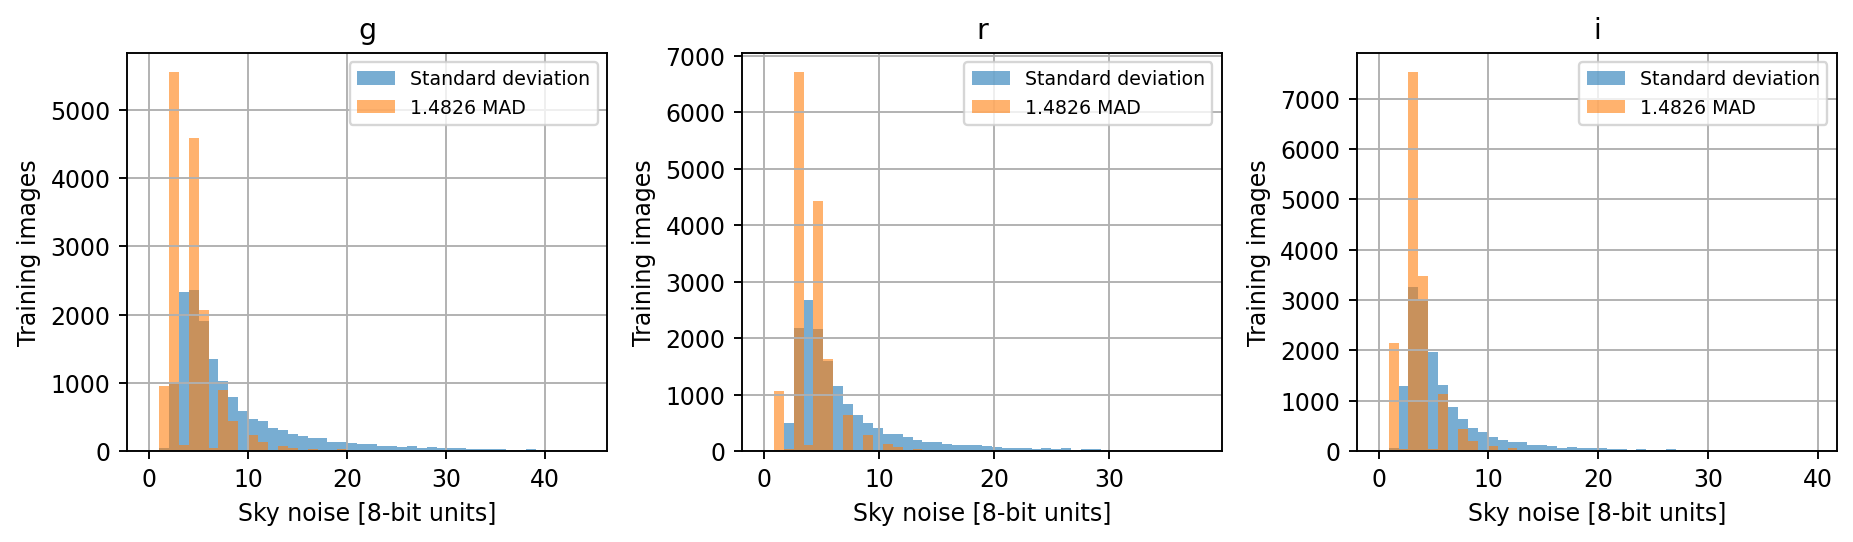
\includegraphics[width=0.94\linewidth,height=150pt,keepaspectratio]{figures/sky_noise.png}
\caption{Training-set distributions of the two sky-noise estimators. The displayed range ends at the 99.5th percentile of the standard deviation; the saved measurements include the tails.}
\label{fig:hw2-2}
\end{figure}

I found median standard deviations of 5.99, 5.21 and 4.51 intensity units in g, r and i. The robust estimates are lower: 4.45, 2.97 and 2.97. Bright border objects or galaxy light can raise the standard deviation more strongly than the MAD, which explains the difference in Fig.~\ref{fig:hw2-2}. These estimates describe fluctuations in the resized, quantised images, rather than calibrated detector noise \cite{ref1}.


\subsubsection*{(b) Signal-to-noise.}

\begin{figure}[H]
\centering
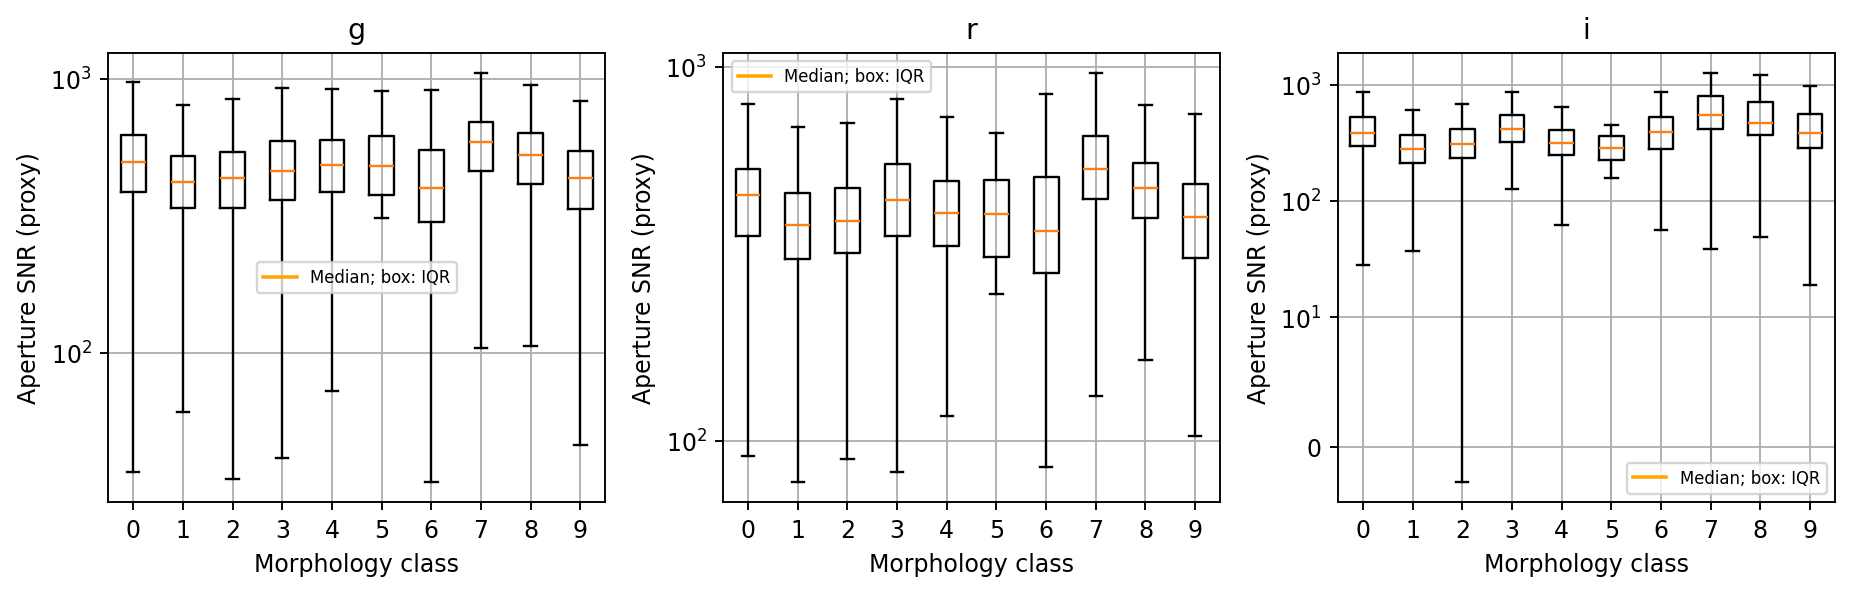
\includegraphics[width=0.94\linewidth,height=155pt,keepaspectratio]{figures/snr.png}
\caption{Aperture SNR proxy by class and band. Boxes show the interquartile range and median, with outliers hidden and a symmetric-log vertical axis.}
\label{fig:hw2-3}
\end{figure}

I summed background-subtracted intensity inside radius 8 pixels (197 pixels) and divided by \ensuremath{\sigma}\textsubscript{sky}\ensuremath{\surd}N. In r, the lowest median is class 6 (363.5), while the highest is class 7 (532.0). Lower aperture SNR need not mean lower total luminosity: a fixed aperture also responds to morphology, angular size and concentration. Zero MAD values use a floor of 1/\ensuremath{\surd}12 intensity units; their fractions are 0.01\%, 0.02\%, 0.03\%. This avoids division by zero but does not restore lost noise information.


\subsubsection*{(c) Contamination and digitisation.}


\begin{figure}[H]
\centering
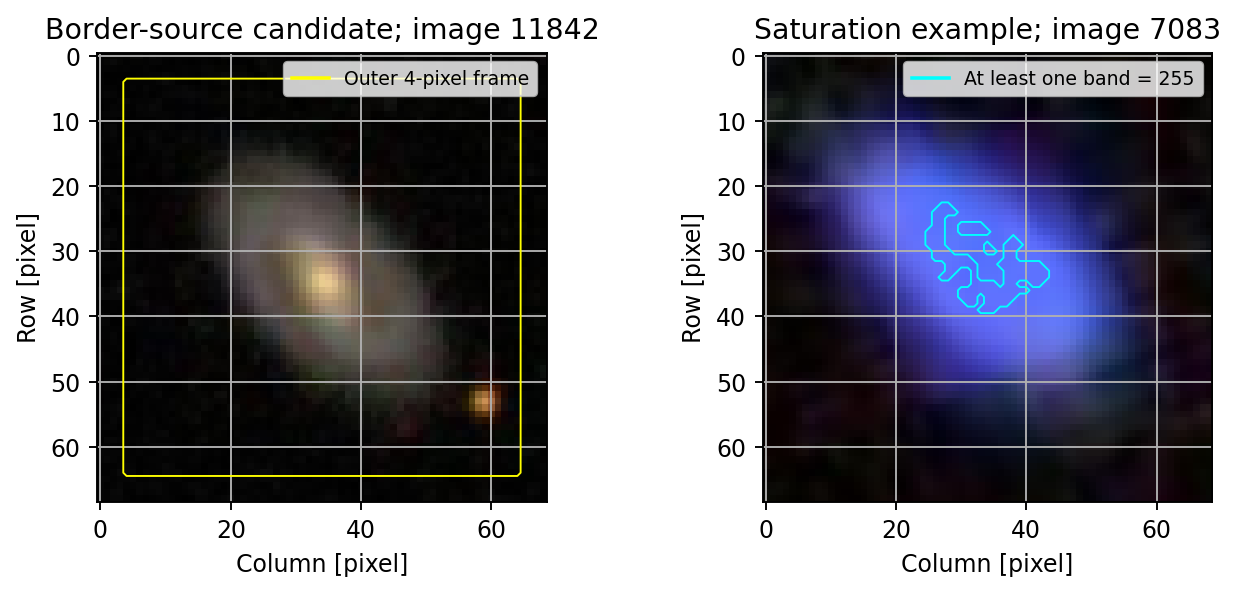
\includegraphics[width=0.94\linewidth,height=170pt,keepaspectratio]{figures/contamination.png}
\caption{A candidate bright border source and an image with saturated pixels. The outlines identify the tested regions.}
\label{fig:hw2-4}
\end{figure}

I flagged a possible border source when at least three connected r-band pixels exceeded the median by five robust standard deviations. This flags 61.54\% of training images, but some may contain galaxy outskirts or artefacts rather than neighbouring stars. I would need to inspect them before interpreting this as a neighbour count. Saturation affects 0.0006\% of all training pixel-band values, and 2.41\% of images have at least one value of 255. Contamination mixes light from different objects; saturation loses the differences between values above the stored maximum. Standardisation does not undo either effect.

\subsubsection*{(d) Label noise.}

I expect confusion between completely round and intermediate smooth galaxies (1 and 2), between adjacent spiral-tightness classes (7, 8 and 9), and between the edge-on bulge classes (4, 5 and 6). The distinctions can become ambiguous when the relevant structure is faint or unresolved. The labels were filtered using volunteer agreement, but agreement is not a guarantee of a correct physical label \cite{ref1}. Label uncertainty limits reliable generalisation to the recorded labels; it does not provide a numerical accuracy ceiling without a model of the errors or repeated independent labels.

The images therefore have several sources of uncertainty: sky noise, possible neighbours, clipping and ambiguous labels. I can subtract a background offset and crop away some contamination, but I cannot recover clipped values or resolve an uncertain label through normalisation. The border-source fraction also depends strongly on my threshold, so I would not treat it as a confirmed contamination rate.


\subsection{Preprocessing pipeline}

\subsubsection*{(a) Crop.}


\begin{figure}[H]
\centering
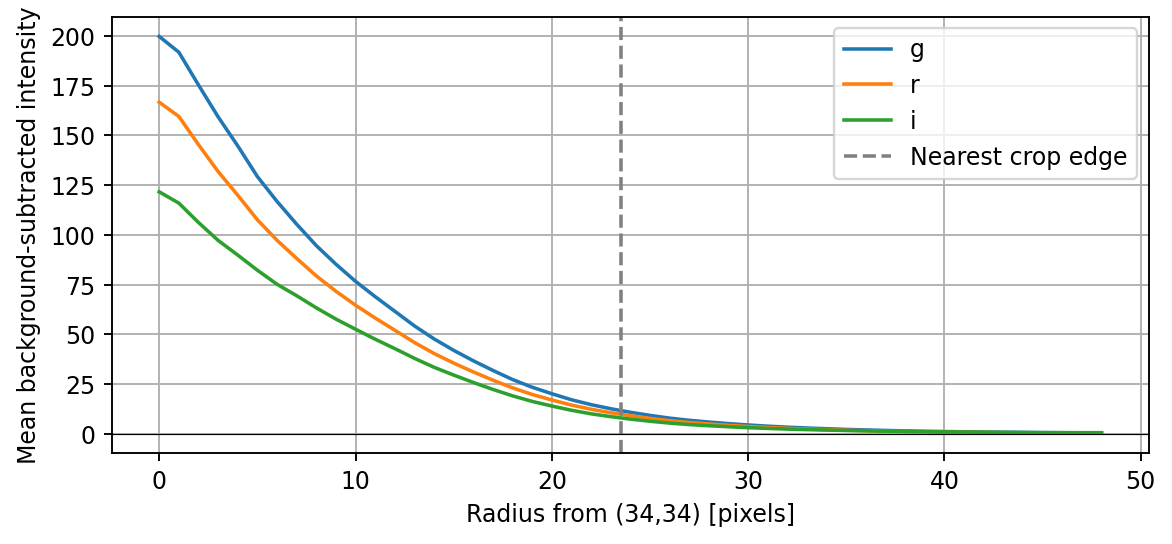
\includegraphics[width=0.94\linewidth,height=155pt,keepaspectratio]{figures/radial_profile.png}
\caption{Mean training-set radial light profile after border-median subtraction. The dashed line marks the nearest edge of the reference crop.}
\label{fig:hw2-5}
\end{figure}

I used rows and columns 10--57 for both models. This retains 88.4\% of the positive background-subtracted intensity, including positive noise and neighbours; it is not a calibrated galaxy-flux fraction. At radius 23 pixels, mean r-band intensity is 10.65, compared with 166.72 at the centre. The crop keeps the bright central structure while reducing sky area, although some outskirts are lost.

\subsubsection*{(b) Normalisation.}

I converted the images to floating point and standardised each band using
\begin{equation}
x'_b=\frac{x_b-\mathrm{sky}_b-\mu_b}{s_b}.
\end{equation}
I calculated $\mu_b$ and $s_b$ from the training crops only and used the same values on validation and test images. Using all images would let held-out information enter the preprocessing, even without their labels.


\begin{table}[H]\centering
\caption{Training-derived normalisation constants and processed moments.}
\small
\begin{tabular}{@{}>{\raggedright\arraybackslash}p{\dimexpr 0.098613\linewidth-4.733pt\relax}>{\raggedright\arraybackslash}p{\dimexpr 0.226823\linewidth-10.888pt\relax}>{\raggedright\arraybackslash}p{\dimexpr 0.226823\linewidth-10.888pt\relax}>{\raggedright\arraybackslash}p{\dimexpr 0.220917\linewidth-10.604pt\relax}>{\raggedright\arraybackslash}p{\dimexpr 0.226823\linewidth-10.888pt\relax}@{}}
\toprule
Band & Training mean \ensuremath{\mu} & Training SD s & Processed mean & Processed SD \\
\midrule
g & 38.8693 & 44.5335 & 3.89e-09 & 1.000000 \\
r & 32.6744 & 37.3249 & -1.86e-08 & 1.000000 \\
i & 26.2158 & 31.6007 & -1.72e-08 & 1.000000 \\
\bottomrule
\end{tabular}
\end{table}


\begin{figure}[H]
\centering
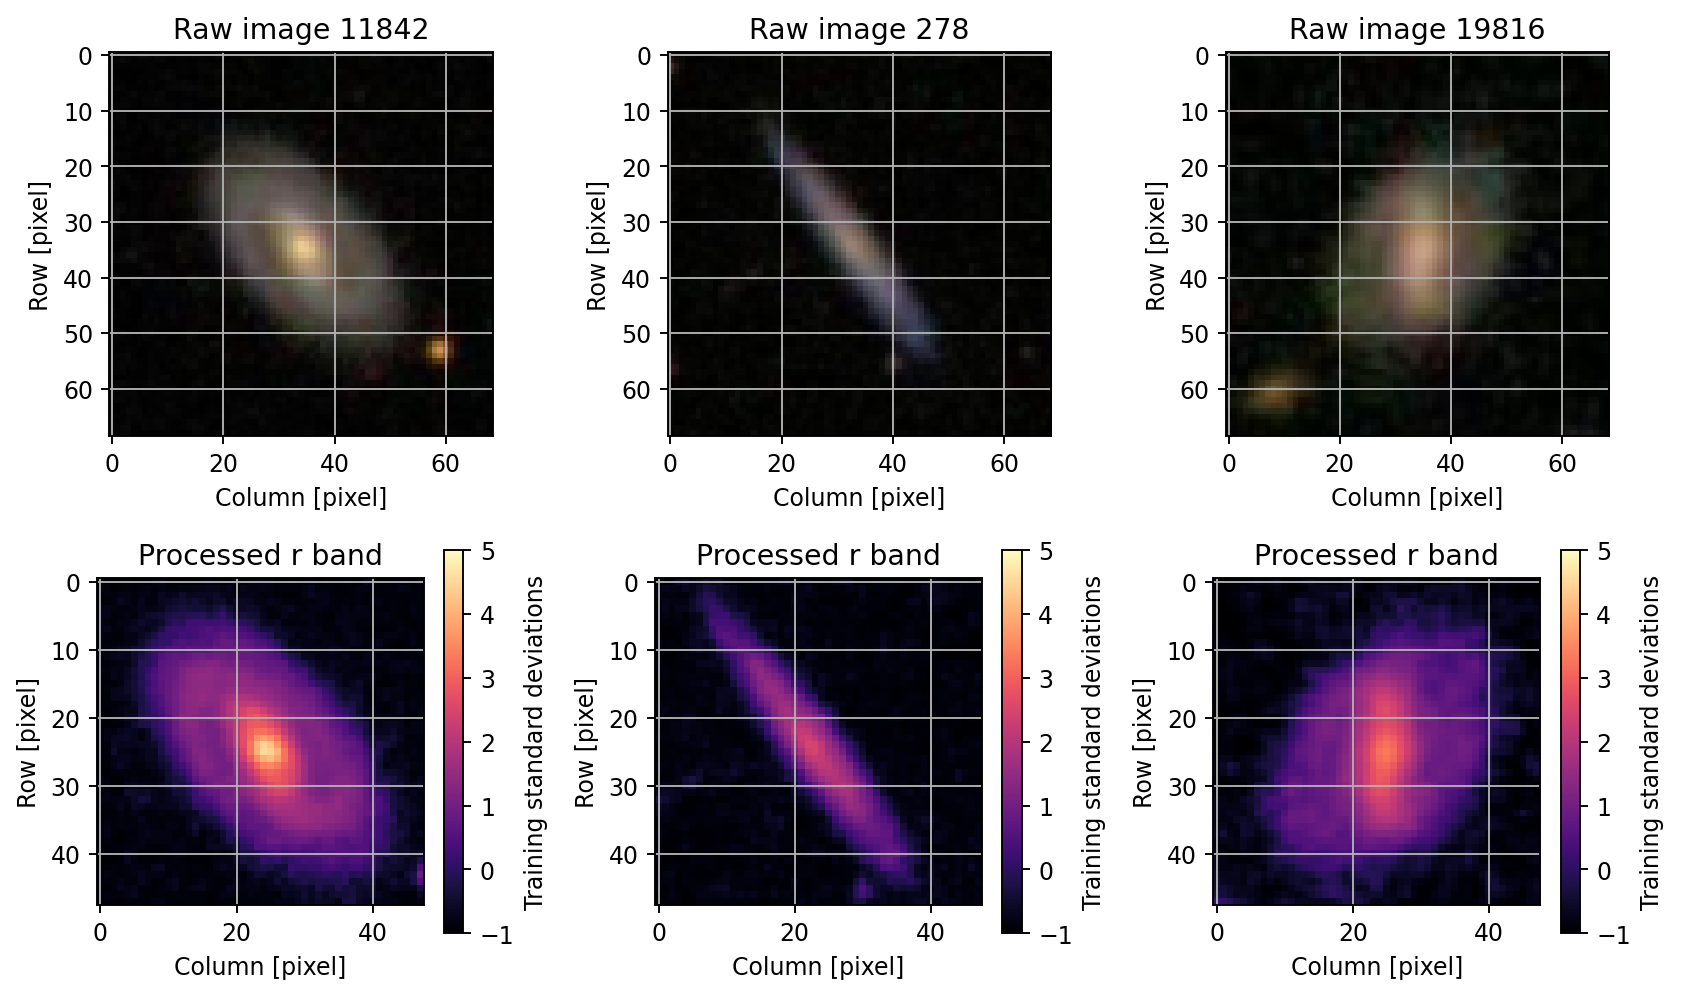
\includegraphics[width=0.94\linewidth,height=200pt,keepaspectratio]{figures/preprocessing.png}
\caption{Raw colour images and their processed r-band crops. The processed panels share a fixed colour scale in training standard deviations.}
\label{fig:hw2-6}
\end{figure}

Dividing each image by its brightest pixel removes its overall amplitude and can make the scale depend on a noisy or saturated pixel. A common divisor preserves relative colours, whereas separate per-band divisors also remove colour ratios. Brightness is not itself the morphology label, but surface brightness and signal-to-noise determine whether spiral structure is measurable. I therefore retained the image intensity scale after additive sky subtraction.

\subsubsection*{(c) Background.}

I subtracted each image's per-band border median; the typical levels are 6.0, 6.0, 3.0 units. This removes an additive offset while preserving the intensity scale. It does not remove random noise or restore clipped values, and galaxy light in the border can bias it.

\subsubsection*{(d) Class imbalance.}

I used class-weighted cross-entropy with weights proportional to $1/\sqrt{n_c}$, calculated from training counts. I did not use a weighted sampler. This gives the rare classes more influence without the very large weight that $1/n_c$ would give the 17-image class. I keep the same weights for every model. Plain accuracy can be dominated by the large classes, so I also report balanced accuracy.

\subsection{Augmentation and the symmetries of the sky}

I would use flips and 90\textdegree{} rotations because they preserve the morphology label and do not need interpolation. Flips reverse spiral handedness, but handedness is not one of the ten labels. Arbitrary rotations are physically reasonable too, although interpolation changes the sampled noise and a finite crop can cut off some of the galaxy.

Small shifts are useful if the galaxy stays inside the crop. I would be more careful with zoom, changes to the g:r:i ratios, and blurring. These change the apparent scale, colour or visibility of the structure, so I would need to justify them as possible observations of the same object.

I would start with flips, 90\textdegree{} rotations and small bounded shifts. I used no augmentation in the baseline or scrambled experiments, keeping the training comparison the same for every model.

\section{FCNN vs. 2D CNN on equal footing}

All models use the identical split, 48 \ensuremath{\times} 48 crops, sky subtraction, training-derived scaling and weighted loss. I used Adam with learning rate 0.001, batches of 128, at most 50 epochs, and early stopping after five epochs without an improvement in validation loss. The best validation-loss weights are restored. Seeds 11, 22 and 33 control initialisation and training order. No architecture-specific tuning or augmentation was used.

I ran all eleven models sequentially on the same Tesla T4 GPU in Colab, using PyTorch 2.11.0+cu130 and NumPy 2.1.3. I synchronised CUDA before each timing measurement. An epoch includes training and validation, but excludes setup, plotting and file writing. Dropout is active when I record training loss and switched off for validation, so part of the gap between the curves also comes from that difference.

The common target is the highest validation accuracy reached by FCNN-matched across its three seeds: 70.13\%. I record the first epoch and cumulative measured epoch time reaching it. Unreached targets are reported explicitly. The representative seed for each confusion matrix and ROC curve is chosen by validation loss, not test accuracy.


\subsection{Baseline comparison}


\begin{table}[H]\centering
\caption{Baseline test performance over three seeds.}
\small
\begin{tabular}{@{}>{\raggedright\arraybackslash}p{\dimexpr 0.220912\linewidth-10.604pt\relax}>{\raggedright\arraybackslash}p{\dimexpr 0.197244\linewidth-9.468pt\relax}>{\raggedright\arraybackslash}p{\dimexpr 0.226818\linewidth-10.887pt\relax}>{\raggedright\arraybackslash}p{\dimexpr 0.177513\linewidth-8.521pt\relax}>{\raggedright\arraybackslash}p{\dimexpr 0.177513\linewidth-8.521pt\relax}@{}}
\toprule
Model & Accuracy (\%) & Balanced accuracy (\%) & Parameters & Best epoch \\
\midrule
FCNN-matched & 68.64 \ensuremath{\pm} 2.54 & 49.16 \ensuremath{\pm} 2.09 & 168,162 & 12.3 \ensuremath{\pm} 1.2 \\
FCNN-large & 70.76 \ensuremath{\pm} 0.68 & 52.99 \ensuremath{\pm} 1.94 & 1,803,914 & 9.3 \ensuremath{\pm} 4.2 \\
CNN & 75.91 \ensuremath{\pm} 1.21 & 59.47 \ensuremath{\pm} 0.11 & 171,754 & 18.3 \ensuremath{\pm} 3.1 \\
\bottomrule
\end{tabular}
\end{table}

I report the mean and sample standard deviation across the three seeds. The best epoch is the one with the lowest validation loss, even though training continues for another five epochs before stopping. The parameter counts in the notebook agree with T1.


\begin{figure}[H]
\centering
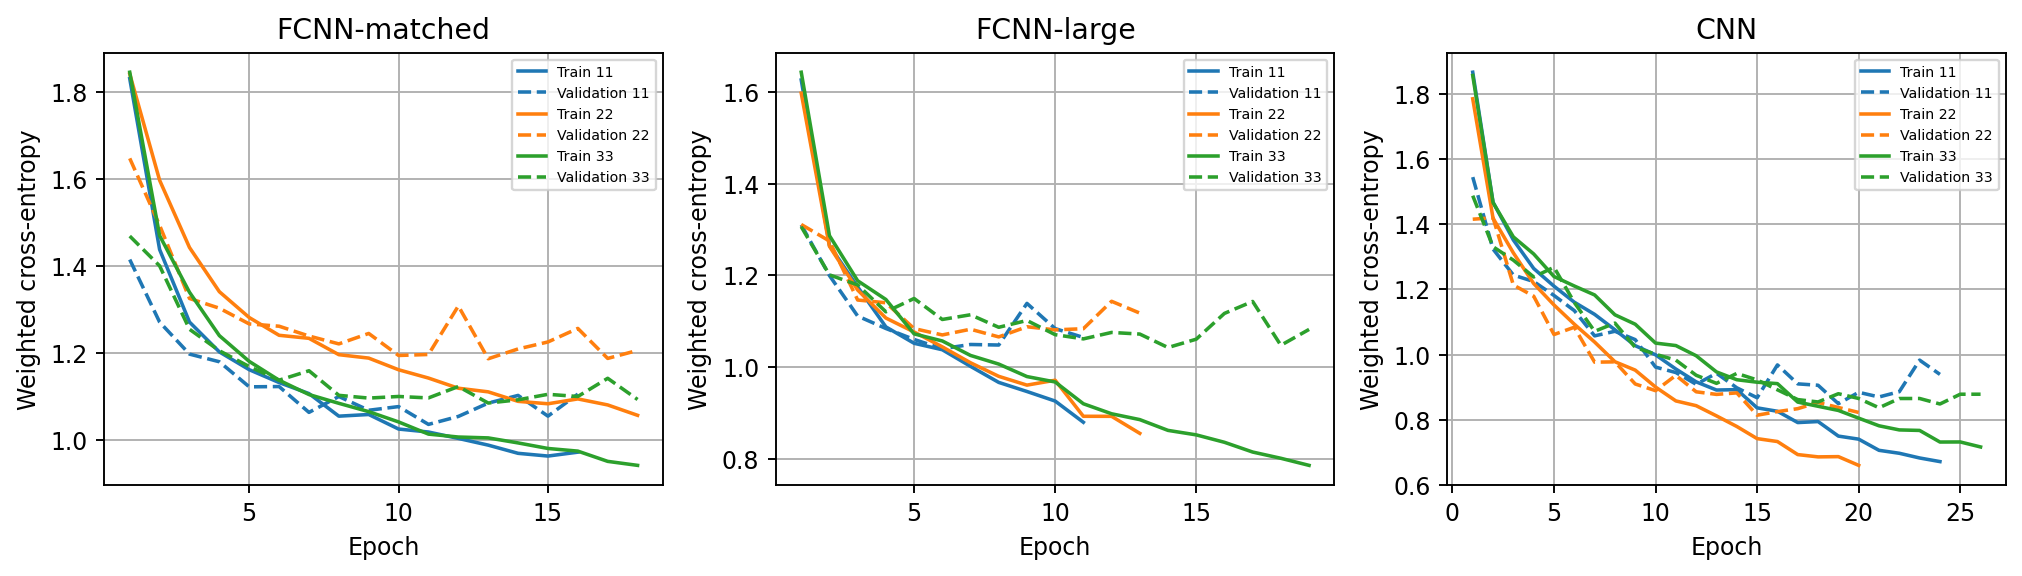
\includegraphics[width=0.94\linewidth,height=205pt,keepaspectratio]{figures/training_curves.png}
\caption{Training and validation weighted cross-entropy for every baseline seed. Solid and dashed lines share a colour within each seed.}
\label{fig:hw2-7}
\end{figure}

The CNN reached $75.91\pm1.21\%$ test accuracy, compared with $68.64\pm2.54\%$ for FCNN-matched and $70.76\pm0.68\%$ for FCNN-large. Its balanced accuracy was also higher: $59.47\pm0.11\%$, compared with $49.16\pm2.09\%$ and $52.99\pm1.94\%$. However, balanced accuracy is well below ordinary accuracy for all three models. The high overall scores therefore hide poorer performance on some of the less common classes.


\begin{table}[H]\centering
\caption{Measured training times and common-target reach counts.}
\footnotesize
\begin{tabular}{@{}>{\raggedright\arraybackslash}p{\dimexpr 0.197241\linewidth-11.944pt\relax}>{\raggedright\arraybackslash}p{\dimexpr 0.163701\linewidth-9.822pt\relax}>{\raggedright\arraybackslash}p{\dimexpr 0.147931\linewidth-8.876pt\relax}>{\raggedright\arraybackslash}p{\dimexpr 0.147931\linewidth-8.876pt\relax}>{\raggedright\arraybackslash}p{\dimexpr 0.173563\linewidth-10.414pt\relax}>{\raggedright\arraybackslash}p{\dimexpr 0.169632\linewidth-10.178pt\relax}@{}}
\toprule
Model & Seconds / epoch & Epochs run & Target reached & Epochs to target* & Seconds to target* \\
\midrule
FCNN-matched & 0.52 \ensuremath{\pm} 0.02 & 17.3 \ensuremath{\pm} 1.2 & 1/3 & 11.0 & 6.2 \\
FCNN-large & 0.55 \ensuremath{\pm} 0.00 & 14.3 \ensuremath{\pm} 4.2 & 3/3 & 11.3 \ensuremath{\pm} 3.8 & 6.3 \ensuremath{\pm} 2.1 \\
CNN & 1.00 \ensuremath{\pm} 0.05 & 23.3 \ensuremath{\pm} 3.1 & 3/3 & 10.3 \ensuremath{\pm} 2.1 & 10.7 \ensuremath{\pm} 2.6 \\
\bottomrule
\end{tabular}
\end{table}

{\footnotesize *Target summaries include only runs that reached the target. A single successful run has no between-seed standard deviation. These conditional times should not be interpreted as the expected time for an arbitrary seed. Individual histories and censored runs are included in the notebook results.\par}

I measured a CNN/FCNN-matched epoch-time ratio of 1.90, much smaller than the forward-MAC ratio of about 38.4. The GPU can perform operations in parallel, and the timings also include memory movement and validation. MAC counts therefore do not translate directly into seconds. This comparison describes the T4 runtime I used; I would need new measurements for another device.

{\footnotesize Individual CNN epochs range from 0.95 to 3.16 seconds (median 0.96). I retained the slow epochs in the reported means and time-to-target values. The same device was used throughout, but these wall-clock measurements include runtime variability and are not isolated hardware benchmarks.\par}

For the validation-selected representative seeds, FCNN-matched selects epoch 11 (validation loss 1.035), then finishes at loss 1.105; FCNN-large selects epoch 6 (validation loss 1.040), then finishes at loss 1.065; CNN selects epoch 15 (validation loss 0.814), then finishes at loss 0.822. Continued training beyond the selected epoch does not improve the selected validation objective, even when the training loss falls. I use the restored checkpoints for every subsequent comparison.


\subsubsection*{Which classes are confused?}


\begin{figure}[H]
\centering
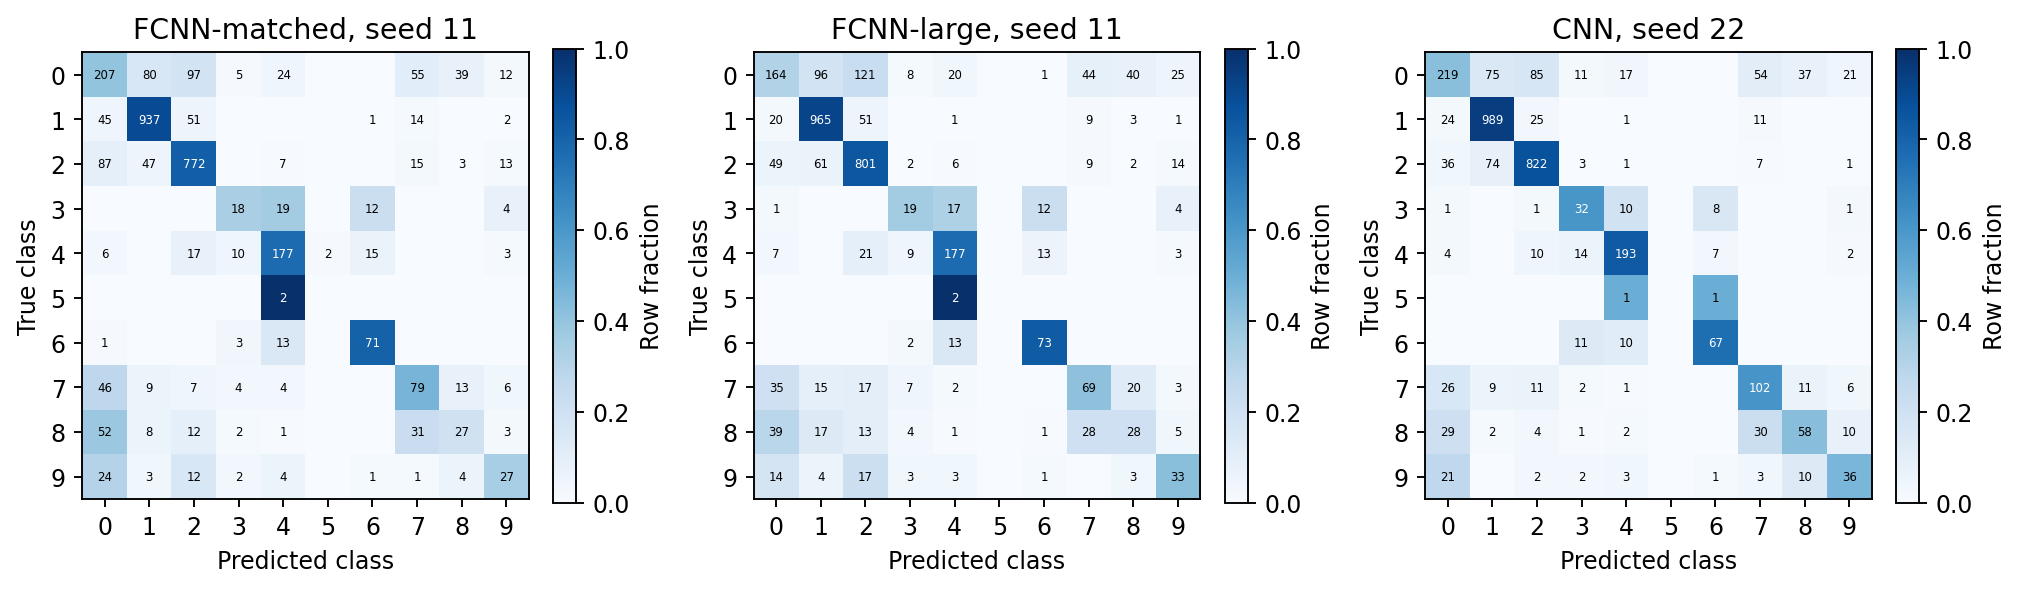
\includegraphics[width=0.94\linewidth,height=430pt,keepaspectratio]{figures/confusion_matrices.png}
\caption{Confusion matrices for the lowest-validation-loss seed of each architecture. Colour is the fraction within each true class; numbers are image counts.}
\label{fig:hw2-8}
\end{figure}

The largest individual mistakes were $0\to2$ (97 images) and $2\to0$ (87) for FCNN-matched; $0\to2$ (121) and $0\to1$ (96) for FCNN-large; and $0\to2$ (85) and $0\to1$ (75) for the CNN. Since the classes have different sizes, I also look at the row-normalised colours rather than comparing counts alone.

The CNN confuses smooth classes 1 and 2 in 99 cases and the spiral classes 7--9 with one another in 70 cases. These are the neighbouring-category confusions anticipated in Section 2.2. Class 0 also lacks visible spiral structure, so confusion with a smooth class can reflect an unresolved distinction between a face-on disk and a smooth object.

For the representative CNN, class 5 has 0 correct predictions out of 2 test examples. A change of one prediction changes that class's recall by 50.0 percentage points and ten-class balanced accuracy by 5.00 points. Repeating training seeds does not remove this uncertainty because all seeds use the same test galaxies.


\subsubsection*{ROC curves}


\begin{figure}[H]
\centering
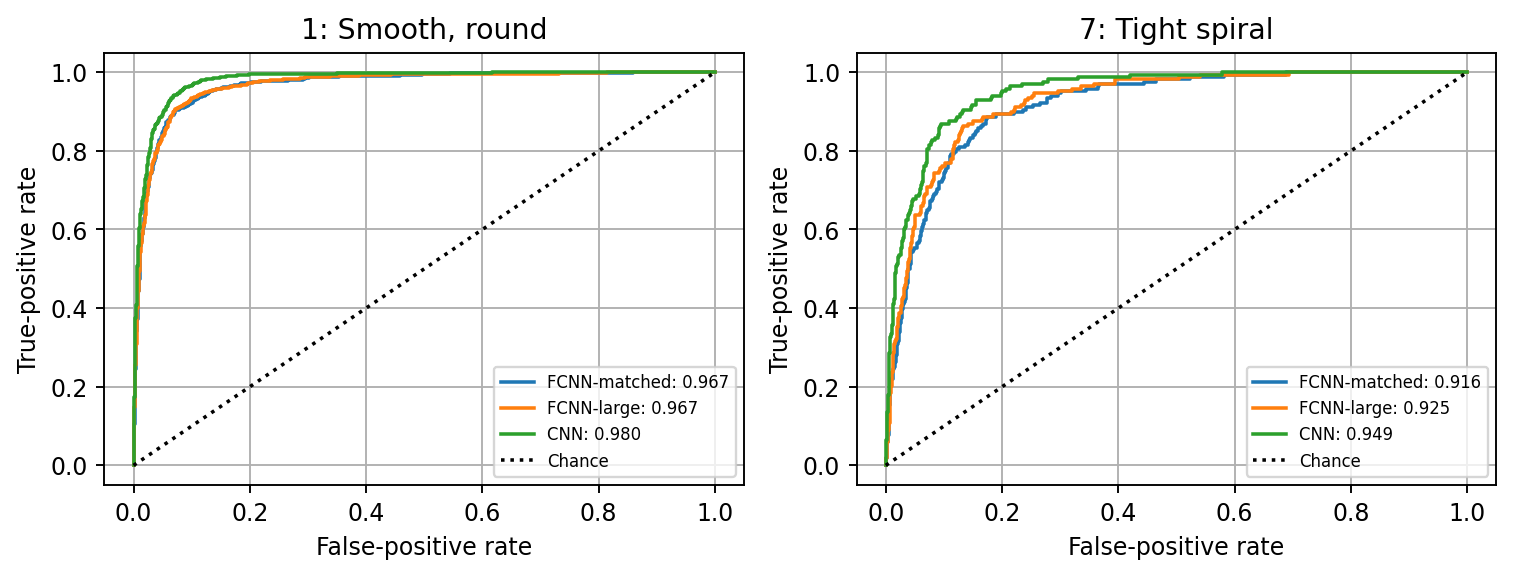
\includegraphics[width=0.94\linewidth,height=205pt,keepaspectratio]{figures/roc.png}
\caption{One-vs-rest ROC curves for a common smooth class (1) and a spiral class (7), using validation-selected seeds.}
\label{fig:hw2-9}
\end{figure}

I used classes 1 and 7 for the ROC curves. These vary the threshold on one class's score, whereas the confusion matrix uses whichever of the ten scores is largest. A good ROC curve therefore does not mean every multiclass decision is correct. The confusions are consistent with faint or ambiguous structure, but I cannot conclude from the matrix alone that the volunteer labels are wrong.

\subsection{Shifted galaxies}


\begin{figure}[H]
\centering
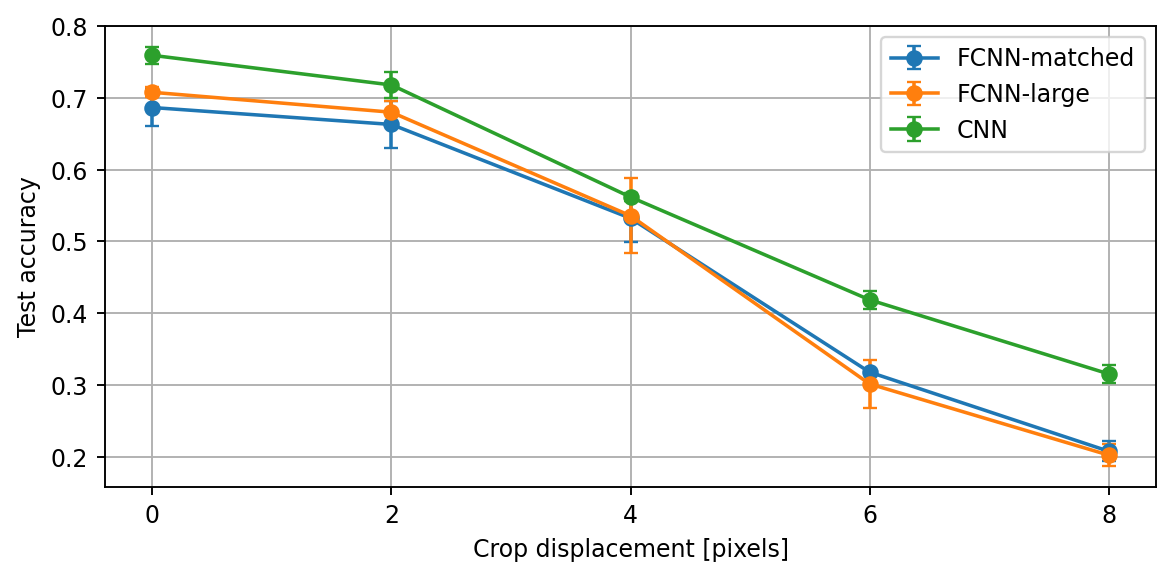
\includegraphics[width=0.94\linewidth,height=190pt,keepaspectratio]{figures/shift_robustness.png}
\caption{Test accuracy under displaced crops. Error bars show the standard deviation across seeds on the same test set.}
\label{fig:hw2-10}
\end{figure}

At an eight-pixel displacement, FCNN-matched: 68.64\% to 20.76\% (47.88 percentage points lost); FCNN-large: 70.76\% to 20.22\% (50.54 percentage points lost); CNN: 75.91\% to 31.53\% (44.38 percentage points lost). Each image receives one fixed random cardinal direction, reused across displacements, models and seeds. The offsets have exactly the requested integer-pixel length. Sky estimates still use the original 69 \ensuremath{\times} 69 border, and the training normalisation is unchanged.

Shifting the crop moves the galaxy within the input, but also changes which outskirts and background pixels remain visible. I therefore interpret this as a practical test of displaced crops. Pooling and shared filters may help with position changes, but the dense head still depends on position, and no model can recover light that has left the crop.

At $d=8$, the CNN retains higher accuracy and loses fewer points than either FCNN. However, at $d=2$ it loses 4.13 points, compared with 2.36--2.77 for the FCNNs. My prediction in T4 was therefore only partly right: the CNN copes better with the larger shifts here, but its advantage is not consistent across all displacements.


\subsection{Scrambled pixels}


\begin{figure}[H]
\centering
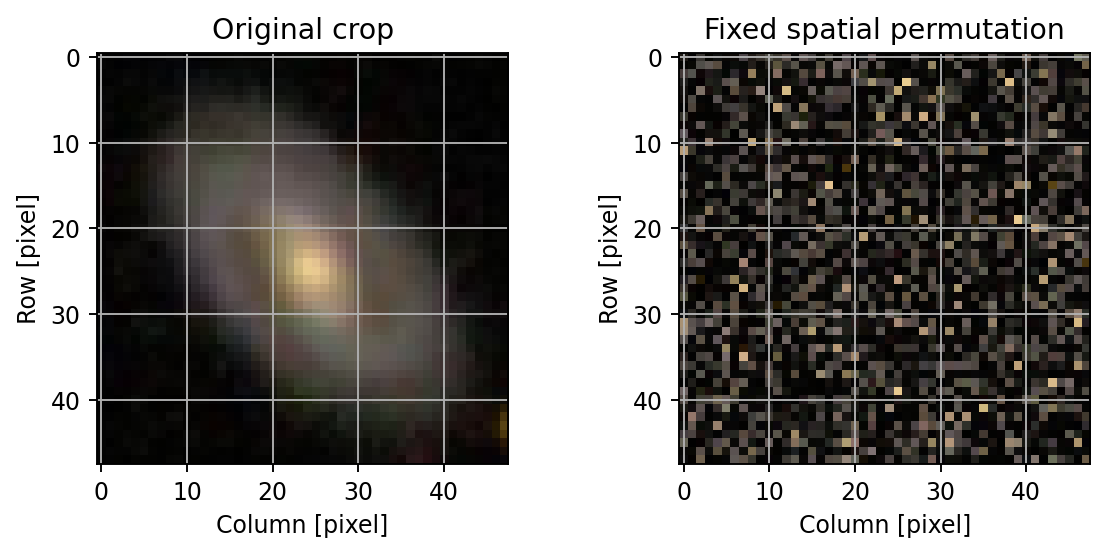
\includegraphics[width=0.94\linewidth,height=220pt,keepaspectratio]{figures/scrambled_example.png}
\caption{One shared permutation reorders 2,304 spatial positions, keeping the three bands together at each position.}
\label{fig:hw2-11}
\end{figure}


\begin{table}[H]\centering
\caption{Original and scrambled test performance for seed 11.}
\small
\begin{tabular}{@{}>{\raggedright\arraybackslash}p{\dimexpr 0.218936\linewidth-10.509pt\relax}>{\raggedright\arraybackslash}p{\dimexpr 0.195266\linewidth-9.373pt\relax}>{\raggedright\arraybackslash}p{\dimexpr 0.195266\linewidth-9.373pt\relax}>{\raggedright\arraybackslash}p{\dimexpr 0.195266\linewidth-9.373pt\relax}>{\raggedright\arraybackslash}p{\dimexpr 0.195266\linewidth-9.373pt\relax}@{}}
\toprule
Model, seed 11 & Original accuracy \% & Scrambled accuracy \% & Original balanced \% & Scrambled balanced \% \\
\midrule
FCNN-matched & 70.84 & 63.28 & 50.40 & 52.35 \\
CNN & 76.04 & 73.75 & 59.56 & 54.14 \\
\bottomrule
\end{tabular}
\end{table}

I retrained both models from scratch using the same fixed permutation in training, validation and test. I compare each with its original seed-11 run. Only one scrambled seed was trained per model, so this experiment does not tell me how variable the scrambling effect is across seeds. Rearranging the FCNN's inputs leaves its representational capacity unchanged, but retraining need not find equivalent weights.

I expected scrambling to hurt the CNN more, but that is not what I found for this seed. CNN accuracy fell by 2.29 points, compared with 7.56 for FCNN-matched. Balanced accuracy changed differently: it fell by 5.43 points for the CNN and increased by 1.95 for the FCNN. I would repeat the experiment with more seeds before drawing a firm conclusion.

The scrambled CNN still performs better than the matched FCNN. All the colour and intensity values remain present, and the CNN retains a dense head containing 85.9\% of its parameters. These may help explain its remaining accuracy, although I have not checked which features it actually uses.


\section*{B2. Robustness to noise.}


\begin{figure}[H]
\centering
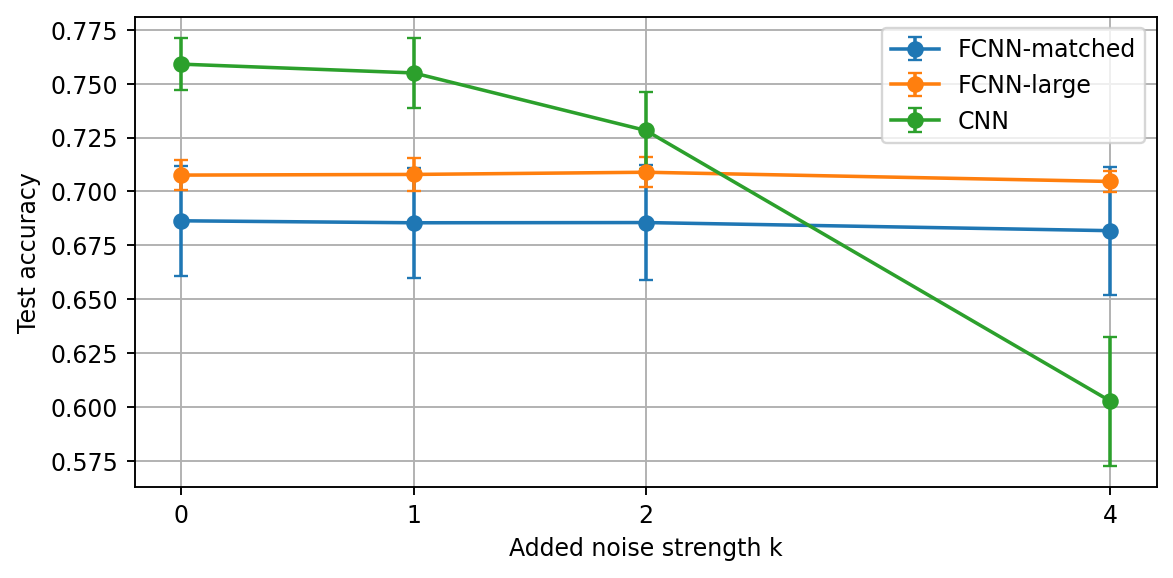
\includegraphics[width=0.94\linewidth,height=160pt,keepaspectratio]{figures/noise_robustness.png}
\caption{Accuracy after adding independent Gaussian noise with standard deviation k times the original robust sky estimate. Error bars show training-seed variation, not independent noise realisations. No models were retrained.}
\label{fig:hw2-12}
\end{figure}

I added Gaussian noise to the raw $69\times69$ test images, using the original robust sky estimate to set its scale. I clipped values to [0,255], estimated the background again, and applied the same crop and training normalisation. I reused the same underlying noise field across strengths and models, without retraining.


\begin{table}[H]\centering
\caption{Test accuracy under added noise.}
\small
\begin{tabular}{@{}>{\raggedright\arraybackslash}p{\dimexpr 0.276138\linewidth-9.941pt\relax}>{\raggedright\arraybackslash}p{\dimexpr 0.246552\linewidth-8.876pt\relax}>{\raggedright\arraybackslash}p{\dimexpr 0.246552\linewidth-8.876pt\relax}>{\raggedright\arraybackslash}p{\dimexpr 0.230757\linewidth-8.307pt\relax}@{}}
\toprule
Model & k = 0 accuracy (\%) & k = 4 accuracy (\%) & Loss (points) \\
\midrule
FCNN-matched & 68.64 \ensuremath{\pm} 2.54 & 68.18 \ensuremath{\pm} 2.97 & 0.46 \\
FCNN-large & 70.76 \ensuremath{\pm} 0.68 & 70.46 \ensuremath{\pm} 0.47 & 0.30 \\
CNN & 75.91 \ensuremath{\pm} 1.21 & 60.26 \ensuremath{\pm} 2.99 & 15.65 \\
\bottomrule
\end{tabular}
\end{table}

At $k=4$, the CNN loses 15.65 accuracy points, compared with 0.46 for FCNN-matched and 0.30 for FCNN-large. The larger FCNN now has the highest accuracy. The CNN's advantage on the original images therefore did not extend to added noise. Max pooling can retain positive fluctuations, as in T7, but this test does not separate pooling from the filters and dense head.

This is a controlled noise test, rather than a full survey model: resizing can correlate pixels, clipping changes the perturbations near 0 and 255, and faint structure becomes harder to see. A learned convolution is also not necessarily an averaging filter. I changed only the test images, keeping the trained models fixed.

\clearpage\section{Discussion}

\textbf{(a)}


\begin{table}[H]\centering
\caption{Comparison of predictive performance and computational cost.}
\footnotesize
\begin{tabular}{@{}>{\raggedright\arraybackslash}p{\dimexpr 0.167660\linewidth-12.071pt\relax}>{\raggedright\arraybackslash}p{\dimexpr 0.149905\linewidth-10.793pt\relax}>{\raggedright\arraybackslash}p{\dimexpr 0.149905\linewidth-10.793pt\relax}>{\raggedright\arraybackslash}p{\dimexpr 0.132151\linewidth-9.515pt\relax}>{\raggedright\arraybackslash}p{\dimexpr 0.151868\linewidth-10.934pt\relax}>{\raggedright\arraybackslash}p{\dimexpr 0.124255\linewidth-8.946pt\relax}>{\raggedright\arraybackslash}p{\dimexpr 0.124255\linewidth-8.946pt\relax}@{}}
\toprule
Model & Accuracy \% & Balanced \% & Params & MACs & s/epoch & s to target* \\
\midrule
Matched FCNN & 68.64 \ensuremath{\pm} 2.54 & 49.16 \ensuremath{\pm} 2.09 & 168,162 & 168,064 & 0.52 \ensuremath{\pm} 0.02 & 6.2 \\
Large FCNN & 70.76 \ensuremath{\pm} 0.68 & 52.99 \ensuremath{\pm} 1.94 & 1,803,914 & 1,803,520 & 0.55 \ensuremath{\pm} 0.00 & 6.3 \ensuremath{\pm} 2.1 \\
CNN & 75.91 \ensuremath{\pm} 1.21 & 59.47 \ensuremath{\pm} 0.11 & 171,754 & 6,451,840 & 1.00 \ensuremath{\pm} 0.05 & 10.7 \ensuremath{\pm} 2.6 \\
\bottomrule
\end{tabular}
\end{table}

{\footnotesize *Mean \ensuremath{\pm} sample SD across seeds where available. Target-time summaries are conditional on reaching the fixed target; reach counts are given in Section 3.1. MACs refer to one forward pass.\par}

The CNN gave me the highest mean accuracy and balanced accuracy. FCNN-large reached the common target in every seed, taking 6.3 seconds on average compared with 10.7 for the CNN. FCNN-matched had the shortest epochs but reached the target in only one of three seeds. The CNN was therefore the most accurate model, while FCNN-large was faster to this particular target on the T4.

\textbf{(b)} Nearby pixels describe structures such as bulges and arms, so I expected the CNN's local filters to help. However, scrambling lowered CNN accuracy by 2.29 points and matched-FCNN accuracy by 7.56 points for seed 11. This did not support my prediction of a larger CNN penalty. Its balanced accuracy fell by 5.43 points, so the effect also depends on how I weight the classes. Stacked convolutions combine information over larger receptive fields, but I did not inspect the filters and cannot claim to have identified the learned features.

The shift experiment partly supported my expectation: the CNN retained 31.5\% accuracy at eight pixels, compared with 20.8\% and 20.2\% for the FCNNs, but its two-pixel drop was larger. Added noise gave the opposite ranking. At $k=4$, the CNN lost 15.65 points while both FCNNs lost less than half a point. The advantage of the CNN therefore depends on how the images change. The sky measurements and aperture SNR also show why architecture alone cannot explain every error.

\textbf{(c)} With only the five magnitudes $u,g,r,i,z$, I would start with an FCNN. There is no two-dimensional image grid for a 2D CNN. The bands have a wavelength order, but they are distinct broad measurements, so moving the same 1D filter between them needs a physical justification.

\textbf{(d)} I would first inspect ambiguous training labels and obtain more examples of the rare classes. Class 5 has only two test galaxies, and several neighbouring categories remain difficult to distinguish. Noise, finite resolution and clipping also limit what the models can see. I would test changes to preprocessing on validation data before adding model complexity, keeping the test set out of those decisions.


\clearpage\section*{AI use}
I used ChatGPT to help me with PyTorch. This is my first time using this library, so I used AI to explain its functions and how to use them. I also used it to do a final organisation of my notebook and the Overleaf document.

\begin{thebibliography}{1}
\bibitem{ref1}
astroNN, ``Galaxy10 SDSS Dataset.'' Dataset definition, class counts, label-vote filtering and image preparation. \href{https://astronn.readthedocs.io/en/latest/galaxy10sdss.html}{Documentation}. Data file: \href{https://zenodo.org/records/10844811/files/Galaxy10.h5}{Galaxy10.h5, Zenodo record 10844811}. Accessed October 14, 2026.

\end{thebibliography}

\end{document}
